% =============================================================================
%  Relatório Técnico — Jogo "Stand"
%  Template SBC (Sociedade Brasileira de Computação) — autocontido
%  Compile com: pdflatex relatorio.tex
% =============================================================================
\documentclass[12pt,a4paper]{article}

% ---- Codificação e idioma ---------------------------------------------------
\usepackage[T1]{fontenc}
\usepackage[utf8]{inputenc}
\usepackage[brazil]{babel}

% ---- Fonte Times (exigida pelo template SBC) --------------------------------
\usepackage{times}

% ---- Margens: 3.5cm topo, 2.5cm base, 3.0cm laterais (SBC) -----------------
\usepackage[top=3.5cm, bottom=2.5cm, left=3.0cm, right=3.0cm]{geometry}

% ---- Utilitários -------------------------------------------------------------
\usepackage{graphicx}
\usepackage{url}
\usepackage{indentfirst}
\usepackage{parskip}       % espaço entre parágrafos em vez de recuo
\usepackage{titlesec}
\usepackage{caption}
\usepackage{float}
\usepackage{microtype}

% ---- Sem cabeçalho, sem rodapé, sem numeração de página (SBC) ---------------
\pagestyle{empty}

% ---- Formatação de seções conforme SBC --------------------------------------
% Seções: negrito 13pt, espaço extra de 12pt acima
\titleformat{\section}{\bfseries\fontsize{13}{15}\selectfont}{\thesection.}{0.5em}{}
\titlespacing*{\section}{0pt}{12pt}{6pt}

% Subseções: negrito 12pt
\titleformat{\subsection}{\bfseries\fontsize{12}{14}\selectfont}{\thesubsection.}{0.5em}{}
\titlespacing*{\subsection}{0pt}{6pt}{3pt}

% ---- Ambientes Abstract / Resumo (SBC) --------------------------------------
\newenvironment{resumo}[1][Resumo]{%
    \par\noindent\textbf{#1.}~\itshape}{\par}

% ---- Configuração de legendas -----------------------------------------------
\captionsetup{font={bf,small},labelfont=bf,justification=centering,skip=6pt}

% =============================================================================
%  INÍCIO DO DOCUMENTO
% =============================================================================
\begin{document}

% ---- Título (16pt, negrito, centralizado) ------------------------------------
\begin{center}
    {\fontsize{16}{20}\bfseries
    Stand: Desenvolvimento de um Jogo de Sobrevivência 3D\\
    com OpenGL e Sistema de Progressão Data-Driven\par}
    \vspace{12pt}

% ---- Autores (12pt, negrito, mesma linha) ------------------------------------
    {\fontsize{12}{14}\bfseries
    Luidge de Sousa Carvalho\textsuperscript{1},
    Samuel Lucas Alves Matos\textsuperscript{1}\par}
    \vspace{6pt}

% ---- Afiliação ---------------------------------------------------------------
    {\fontsize{12}{14}\selectfont
    \textsuperscript{1}%
    %TODO: substitua pelo nome do departamento e universidade
    Departamento de Ciência da Computação —
    [Nome da Universidade]\par}
    \vspace{4pt}

    {\fontsize{10}{12}\ttfamily
    %TODO: substitua pelas matrículas reais
    \{matricula\_luidge, matricula\_samuel\}@[dominio.edu.br]\par}
\end{center}

\vspace{10pt}

% ---- Abstract (inglês) -------------------------------------------------------
\noindent
\begin{minipage}[t]{\dimexpr\linewidth-1.6cm}
    \hspace{0.8cm}%
    \begin{minipage}[t]{\dimexpr\linewidth-0.8cm}
        \fontsize{12}{14}\selectfont
        \textbf{Abstract.} This paper describes the development of
        \textit{Stand}, a 3D top-down survival shooter built with C++ and
        OpenGL without the use of external game engines.
        The work covers a data-driven skill and weapon specialisation system,
        five classes of enemy with dedicated artificial intelligence, an
        adaptive spawn difficulty curve, a boss-fight event driven by a
        finite-state machine, isometric camera projection, collision detection
        with a spatial hash grid, skeletal animation loaded via Assimp, and a
        prioritised audio system using the Windows MCI API.
        The implementation demonstrates core real-time computer graphics
        concepts including geometric transformations, depth testing,
        alpha-blending, orthographic HUD overlay and particle effects.
    \end{minipage}
\end{minipage}

\vspace{8pt}

% ---- Resumo (português) ------------------------------------------------------
\noindent
\begin{minipage}[t]{\dimexpr\linewidth-1.6cm}
    \hspace{0.8cm}%
    \begin{minipage}[t]{\dimexpr\linewidth-0.8cm}
        \fontsize{12}{14}\selectfont
        \textbf{Resumo.} Este artigo descreve o desenvolvimento de
        \textit{Stand}, um jogo de tiro e sobrevivência 3D em perspectiva
        isométrica, construído com C++ e OpenGL sem o uso de \textit{engines}
        externas.
        O trabalho abrange um sistema de habilidades orientado a dados,
        especialização de armas por arquétipos, cinco classes de inimigos com
        inteligência artificial dedicada, curva adaptativa de dificuldade,
        evento de chefe controlado por máquina de estados, câmera isométrica,
        detecção de colisão com grade espacial, animação esqueletal carregada
        via Assimp e sistema de áudio com prioridade de voz via Windows MCI.
        A implementação demonstra conceitos fundamentais de computação gráfica
        em tempo real: transformações geométricas, teste de profundidade,
        \textit{alpha-blending}, HUD ortográfico e efeitos de partículas.
    \end{minipage}
\end{minipage}

% =============================================================================
\section{Introdução}
% =============================================================================

\textit{Stand} é um jogo de sobrevivência 3D em perspectiva isométrica onde
o jogador controla Sofia, uma sobrevivente que combate hordas de zumbis em
uma balada abandonada.
Acompanha-a o \textit{Stand}, uma entidade fantasmagórica que orbita a
personagem e executa ataques configuráveis por meio de um catálogo de
habilidades orientado a dados.

O objetivo da partida é sobreviver ao maior número de ondas possível,
coletando pontos de experiência (XP), evoluindo de nível e especializando o
arsenal.
Após quatro minutos de jogo, o \textit{spawn} de inimigos é bloqueado e, uma
vez que a arena esteja vazia, o Chefe aparece para o confronto final.
Derrotá-lo encerra o ciclo do evento, e a partida retoma os \textit{spawns}
infinitamente em modo de sobrevivência livre.

A motivação do projeto foi explorar técnicas clássicas de computação gráfica
3D em tempo real usando exclusivamente o OpenGL no modo imediato, sem
\textit{engines} externas, desenvolvendo do zero a lógica de jogo, os
sistemas visuais e a interface.

% =============================================================================
\section{Materiais}
% =============================================================================

A Tabela~\ref{tab:materiais} lista as principais ferramentas e bibliotecas
utilizadas e sua finalidade no projeto.

\begin{table}[H]
\caption{Ferramentas e bibliotecas utilizadas}
\label{tab:materiais}
\centering
\begin{tabular}{|l|p{9cm}|}
\hline
\textbf{Tecnologia} & \textbf{Finalidade} \\
\hline
C++ (98/11) & Linguagem principal; compatibilidade com compiladores legados \\
\hline
OpenGL (modo imediato) & Renderização 3D: geometria, transformações, iluminação e \textit{blending} \\
\hline
GLUT & Criação de janela, \textit{loop} principal e callbacks de entrada \\
\hline
Assimp & Carregamento de modelos 3D animados (.glb) — personagem Sofia e pistola \\
\hline
GLM & Matemática de matrizes e vetores para transformações e animação esqueletal \\
\hline
stb\_image & Decodificação de texturas PNG para os modelos carregados via Assimp \\
\hline
Windows MCI & Sistema de áudio: música de fundo em \textit{loop}, efeitos sonoros e falas da protagonista \\
\hline
\end{tabular}
\end{table}

% =============================================================================
\section{Métodos}
% =============================================================================

\subsection{Arquitetura do Projeto}

O projeto adota uma arquitetura modular baseada em \textit{headers} com
responsabilidades bem definidas:
\texttt{entities.h} declara as estruturas de dados POD (\textit{Plain Old
Data}) —\ \texttt{Jogador}, \texttt{Zumbi}, \texttt{EstadoDoJogo} e
\texttt{FasePartida};
\texttt{GameLogic.h} contém a lógica de \textit{spawn}, IA, colisões e
progressão;
o conjunto \texttt{SkillManager/SkillExecutor/SkillCatalog} implementa o
motor de habilidades orientado a dados;
e \texttt{Main.cpp} concentra o \textit{loop} principal, renderização
OpenGL e os \textit{callbacks} GLUT.

\subsection{Movimentação e Câmera}

O jogador move-se com as teclas WASD no plano XZ.
A câmera isométrica segue Sofia a uma distância fixa, posicionada atrás e
acima com inclinação de aproximadamente 45\textdegree\ via
\texttt{gluLookAt}.
A posição do cursor no mundo 3D é obtida por
\texttt{gluUnProject} sobre o \textit{depth buffer}, projetando o
ponteiro do mouse no plano $y = 0$.
O \textit{Stand} posiciona-se diametralmente oposto à direção de mira,
mantendo distância fixa nas costas de Sofia.

\subsection{Inteligência Artificial dos Inimigos}

Os inimigos implementam uma máquina de estados finitos (FSM) com os estados
\texttt{WANDER} e \texttt{CHASE}.
Em \texttt{CHASE}, cada zumbi calcula o vetor normalizado até Sofia e aplica
deslocamento proporcional à sua velocidade por \textit{delta time}.
O Atirador mantém uma distância preferida, recuando quando muito próximo e
avançando quando distante, e dispara projéteis em linha reta.
O Explosivo causa dano em área ao morrer.
Cinco tipos de zumbi estão disponíveis, cada um com atributos distintos de
velocidade, vida e dano (Tabela~\ref{tab:zumbis}).

\begin{table}[H]
\caption{Tipos de inimigos e atributos}
\label{tab:zumbis}
\centering
\begin{tabular}{|l|c|c|c|}
\hline
\textbf{Tipo}    & \textbf{Vida} & \textbf{Velocidade} & \textbf{Dano} \\
\hline
Normal    &  2 & 8.0  & 1 \\
Rápido    &  1 & 10.0 & 1 \\
Tank      & 10 & 5.0  & 3 \\
Atirador  &  2 & 6.0  & 3 \\
Explosivo &  2 & 10.0 & 3 \\
\hline
\end{tabular}
\end{table}

\subsection{Sistema de Colisão}

Colisões entre entidades usam testes de círculos no plano XZ —\ distância
euclidiana menor que a soma dos raios indica contato.
Para a detecção de colisão entre projéteis e inimigos, uma grade espacial
(\texttt{SpatialGrid}) particiona o espaço em células de tamanho fixo,
reduzindo as verificações de $O(n \cdot m)$ para $O(1)$ amortizado por
projétil.

\subsection{Sistema de Progressão e Arquétipos}

O motor de habilidades é totalmente \textit{data-driven}: cada habilidade
é registrada no catálogo como combinação de \textbf{forma} (bloco, círculo,
arco, míssil), \textbf{movimento} (linear, orbital, estático) e
\textbf{efeitos} (perfuração, área, cadência).
O jogador equipa até seis habilidades simultâneas.

O sistema de Arquétipos adiciona uma camada de especialização irreversível:
quando dois atributos diferentes da arma base atingem o nível~2, a arma
se especializa em um dos seis arquétipos disponíveis —\ por exemplo,
\textit{Rifle Laser} (Dano + Perfuração) ou
\textit{Metralhadora Pesada} (Cadência + Dano) —\ bloqueando os demais
atributos pelo restante da partida.

\subsection{Sistema de Boss e Máquina de Estados da Partida}

O progresso da partida é controlado por um \textit{enum} \texttt{FasePartida}
com quatro estados:

\begin{itemize}
    \item \textbf{FASE\_NORMAL:} \textit{spawn} adaptativo de zumbis;
    \item \textbf{FASE\_AGUARDANDO\_BOSS:} ativada aos 4 minutos; novos
          \textit{spawns} são bloqueados; HUD exibe contador de inimigos
          restantes;
    \item \textbf{FASE\_BOSS:} ativada ao zerar a arena; Chefe é invocado;
    \item \textbf{FASE\_VITORIA:} Boss derrotado; \textit{spawn} retoma
          infinitamente; nenhum novo Boss pode surgir.
\end{itemize}

O Boss é representado como um \texttt{Zumbi} especial com o campo
\texttt{ehBoss = true}, inserido no vetor \texttt{g\_jogo.horda}.
Essa decisão de projeto permite que ele reutilize sem modificações os sistemas
de colisão projetil-inimigo, aplicação de dano e IA de perseguição já
existentes.
Seus atributos são centralizados em constantes de fácil ajuste:
5.000 pontos de vida, 5 de dano por contato e velocidade equivalente a 80\%
do zumbi Rápido.
Visualmente, o Chefe exibe um bloco roxo aproximadamente cinco vezes maior
que um zumbi comum, coroa de espigões dourados, olhos vermelhos e uma aura
pulsante no chão.
Uma barra de vida dedicada é exibida no topo da tela durante a batalha.

\subsection{Mecânicas Especiais}

\textbf{Devorar:} ao pressionar \texttt{ESPAÇO}, Sofia executa um ataque
corpo-a-corpo que mata instantaneamente um inimigo ou destrói um projétil
dentro de um setor angular frontal.
Acertar elimina toda a tensão acumulada; errar provoca sobrecarga imediata.

\textbf{Parry:} a tecla \texttt{Q} ativa uma janela de 0,25 s.
Se um inimigo estiver próximo nesse intervalo, todos os zumbis no raio de 15
unidades são repelidos e a tensão é zerada.

\textbf{Tensão:} atirar aumenta a barra de tensão do Stand.
Ao atingir 100\%, a personagem entra em sobrecarga e não pode disparar até a
barra esvaziar, forçando o jogador a gerenciar o ritmo de combate.

\subsection{Sistema de Áudio}

A música de fundo é gerenciada com um \textit{alias} MCI dedicado em
\textit{loop} contínuo.
Efeitos sonoros usam um pool rotativo de dez canais (\texttt{sfx\_0..9}).
As falas da protagonista utilizam um canal exclusivo (\texttt{sfx\_fala}),
isolado do pool, garantindo que sons de zumbis nunca interrompam o diálogo.
A função \texttt{personagemEstaFalando()} consulta o estado MCI do canal para
bloquear sons ambiente enquanto ela estiver falando.

\subsection{Renderização}

O jogo usa OpenGL no modo imediato.
Os zumbis e o Boss são renderizados como blocos 3D coloridos por tipo
(\texttt{GL\_QUADS}).
Sofia é carregada via Assimp (.glb com esqueleto e animações), texturizada
com stb\_image e renderizada com iluminação básica (\texttt{GL\_LIGHT0}).
O HUD é desenhado em modo ortográfico 2D (empilhando e restaurando matrizes
de projeção/modelagem) com barras de HP, XP, tensão e, durante o Boss, barra
de vida na parte superior da tela.
Efeitos de partículas com gravidade e \textit{alpha-blending} são usados
para morte de inimigos.

% =============================================================================
\section{Resultados e Discussão}
% =============================================================================

%TODO: insira aqui capturas de tela do jogo (substitua os nomes de arquivo)
% Sugestão de capturas:
%   - Arena com horda de zumbis e HUD visível
%   - Menu de Level-Up com as três opções
%   - Boss na arena com barra de vida no topo
%   - Tela de Game Over

% Exemplo de inserção de figura (descomente e ajuste o caminho):
%\begin{figure}[H]
%    \centering
%    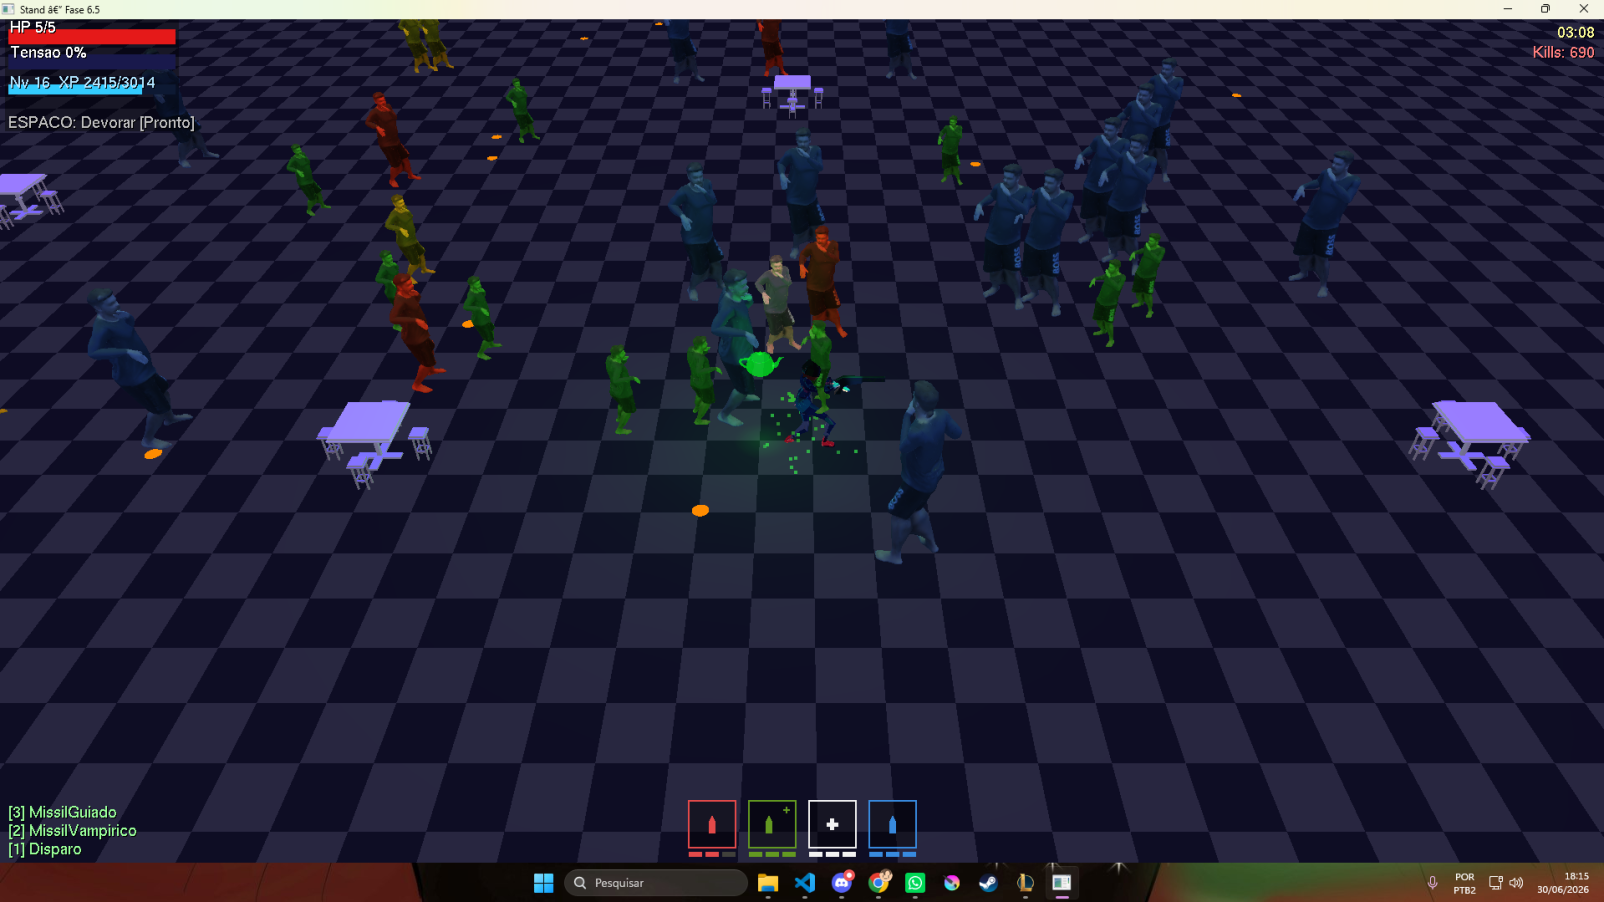
\includegraphics[width=0.9\linewidth]{screenshots/gameplay.png}
%    \caption{Cena de gameplay: Sofia cercada por zumbis com HUD ativo.}
%    \label{fig:gameplay}
%\end{figure}

O jogo executa de forma fluida com até 1.500 zumbis simultâneos, graças à
grade espacial que evita testes de colisão em $O(n^2)$.
O sistema de \textit{spawn} adaptativo dobra a quantidade de inimigos por
minuto por tipo, criando uma curva de dificuldade orgânica.
A diversidade de builds possíveis —\ seis arquétipos com cinco níveis cada
—\ prolonga o \textit{replay}.
A batalha do Boss introduz tensão e um clímax narrativo claro, diferenciando
a estrutura do jogo de \textit{loops} de sobrevivência tradicionais.

Um ponto observado durante os testes foi que o balanceamento de atributos
(vida do Boss, cadência de \textit{spawn}, XP por inimigo) requereu diversas
iterações.
A centralização desses valores em constantes (\texttt{BOSS\_VIDA\_MAXIMA},
\texttt{SPAWN\_BASE}, etc.) facilitou os ajustes sem recompilar módulos
críticos.

% =============================================================================
\section{Conclusão}
% =============================================================================

O projeto atingiu seus objetivos: um jogo de sobrevivência 3D funcional,
com sistema de progressão expressivo e batalha de Boss, implementado
inteiramente com OpenGL e C++ sem engines externas.

Os principais desafios enfrentados foram:
\textbf{(1)} Integrar animação esqueletal (Assimp/GLM) com o \textit{loop}
de renderização OpenGL em modo imediato, exigindo cálculo manual de matrizes
de \textit{bone socket} para ancorar a pistola à mão da personagem;
\textbf{(2)} Projetar o sistema de Boss sem duplicar código de colisão —\
resolvido inserindo o Boss como um \texttt{Zumbi} especial com
\texttt{ehBoss = true} dentro do vetor \texttt{horda}, reutilizando toda a
pipeline existente;
\textbf{(3)} Garantir prioridade de áudio das falas da protagonista sobre
sons de zumbi —\ resolvido com um canal MCI dedicado (\texttt{sfx\_fala})
e consulta de estado via \texttt{mciSendString("status sfx\_fala mode")}.

Como trabalhos futuros, propõe-se: múltiplos tipos de Chefe com padrões de
ataque distintos; sistema de \textit{save} de progressão entre sessões;
suporte a Linux/macOS substituindo o MCI por OpenAL; e modo cooperativo
local com câmera compartilhada.

% =============================================================================
\section*{Referências}
% =============================================================================

\fontsize{12}{14}\selectfont

\noindent
OpenGL Architecture Review Board (2004). \textit{OpenGL Reference Manual},
4th ed. Addison-Wesley.
URL: \url{https://www.opengl.org/documentation/}

\vspace{6pt}\noindent
Kilgard, M. J. (1996). \textit{The OpenGL Utility Toolkit (GLUT) Programming
Interface}. Silicon Graphics.
URL: \url{https://www.opengl.org/resources/libraries/glut/}

\vspace{6pt}\noindent
Assimp Development Team (2023). \textit{Open Asset Import Library (Assimp)}.
URL: \url{https://assimp.org/}

\vspace{6pt}\noindent
G-Truc Creation (2023). \textit{OpenGL Mathematics (GLM)}.
URL: \url{https://glm.g-truc.net/}

\vspace{6pt}\noindent
Barrett, S. (2017). \textit{stb\_image — Single-file public domain image
loader library}.
URL: \url{https://github.com/nothings/stb}

\vspace{6pt}\noindent
Microsoft Corporation (2023). \textit{MCI Command Strings — Windows Multimedia}.
URL: \url{https://docs.microsoft.com/en-us/windows/win32/multimedia/mci-command-strings}

\vspace{6pt}\noindent
Shreiner, D. \textit{et al.} (2013). \textit{OpenGL Programming Guide}, 8th ed.
Addison-Wesley.

\end{document}
